\chapter{Konzept}
\label{chap:konzept}


\section{Allgemein}

\textbf{Gateway} \\
Die einzelnen Sensoren eines \gls{iot} Systems sind an einen Gateway angeschlossen. Dies kann fix per Kabel oder über eine Drahtlosschnittstelle wie z. Bsp. Bluetooh umgesetzt sein. Typsicherweise werden Kleincomputer (Single Board Computer) wie ein Raspberry Pi oder Intel Galileo eingesetzt. Diese Geräte zeichen sich aus durch sehr kompakte Bauform (Kreditkatenformat) und bieten trotzdem genügend Ressourcen um darauf Hardwareunahängige Anwendungen (z. Bsp. Java, Python, Javascript) laufen zu lassen. 
Ein Gateway führt die Daten der einzlenen Sensoren zusammen führt einheiltliche Formate der Daten ein. Ausserdem übernimmt er die Kommunikation mit der Aussenwelt, indem er eine Verbindung zum zentralen Broker herstellt.

\textbf{Broker} \\
Der Broker ist bei \acrshort{a_mqtt} Anwendungen von zentraler Bedeutung, da alle Daten via Broker zwischen den Teilnehmern ausgetauscht werden. Pro System gibt es typischeise einen Broker. Dieser muss für alle Teilnehmener (Gateways und Applikationen) einfach zu erreichen sein und muss eine hohe Verfügbarkeit aufweisen.

\textbf{Application} \\
Es können grundsätzlich beliebige Appliaktionen auf allen gängigen Platformen und Technologien mit den System kommunizieren. Die einzige Grundbedingung ist, dass die Applikation \acrshort{a_mqtt} fähig ist, was sich durch das Einbinden der entsprechenden Libraries einfach realisieren lässt.
\\


Bei der Beschreibung eines einzelnen Devices werden folgende drei Bereiche unterschieden:

\textbf{State} \\
Die Menge aller Eigenschaften des Devices und deren Werte wird als State bezeichnet. Beispielsweise Name, Firmwareversion, etc. Der State eines Devices ist beständig, d.h. solange keine Interaktion geschieht, verändert sich der State nicht.


\textbf{Events} \\
Tritt auf dem Device ein Ereignis ein, wird dadurch ein Event erzeugt. Ein Event wird grundsätzlich vom Device selbst ausgelöst. Beispielsweise erzeugt ein Temperatursensor alle 5 Sekunden ein Event welches den Messwert enthält. Applikationen registrieren sich, um bestimmte Events von den Devices zu erhalten.


\textbf{Commands} \\
Eine Anwendung interagiert mit einem Device, indem Commands an eines oder mehrere Devices gesendet werden. Die Devices empfangen die Commands und reagieren entsprechend. Ein Command ist bestimmt durch einen Namen und Parameter mit dazugehörigen Werten. 
Beispielsweise kann bei einem Temperatursensor über einen Command \code{SetInterval: 10s} der Abstand der Messungen eingestellt werden.
Ein Device muss bekanntgeben, auf welche Commands mit welchen Paramtern es reagiert.


\begin{figure}[H]
	\centering
		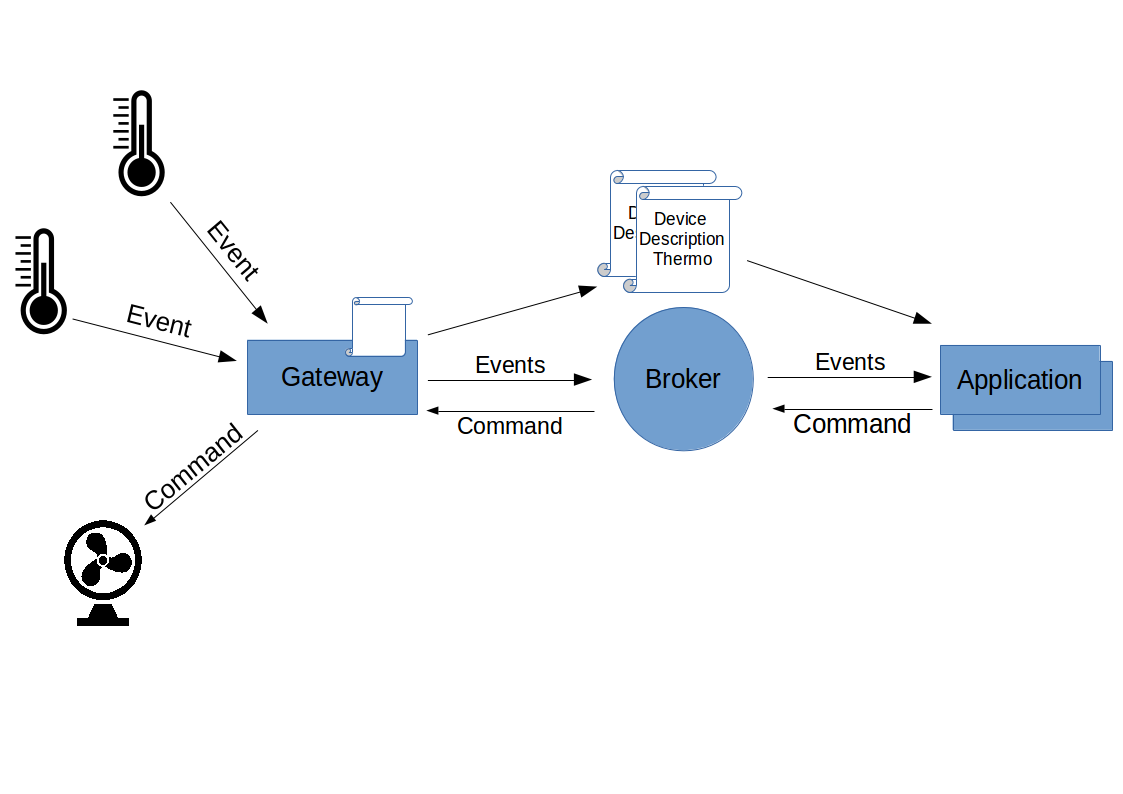
\includegraphics[width=0.8\textwidth]{diag/Overview.png}
	\caption{\label{fig:overview}Übersicht der}
\end{figure}


\section{Hierarchie Topics}


Die Topic Hiearachie wird nach folgenden Muster aufgebaut:


\begin{table}[h!]
\begin{tabularx}{\textwidth}{|l|X|l|}

 \hline
 {\bf Level } & {\bf Beschreibung } & {\bf Beispiel } \\ 
 \hline
 0  &   \textbf{Identifikation Anwendung} \newline Eindeutige identifikation der Anwendung.  &    
  ch.bfh.barta3.myApp   \\ \hline
 
 1  &   \textbf{Master Host}  \newline Gruppierung der Devices auf Stufe 1  &     -   \\ \hline

 2  &   \textbf{Host} \newline Gruppierung der Devices auf Stufe 2   &   -   \\ \hline

 3  &   \textbf{Device Typ} \newline Bezeichnung, um was für einen Typ von Sensor oder Aktor es sich handelt.  &     Temperatursensor   \\ \hline

 4  &   \textbf{Device ID} \newline Da mehrere Devices vom selben Typ im Einsatz sein können, wird auf dieser Stufe mit einer eindeutigen ID der konkrete Sensor resp. Aktor angegeben.   &    mxg   \\ \hline
 
  4  &   \textbf{Device Description} \newline d   &    -   \\ \hline

 5  &   \textbf{Kategorisierung Devicedaten} \newline  Die Eigenschaften und Daten werden in die nachfolgenden drei Teile aufgegliedert.  &     Events, State, Commands   \\ \hline

 6  &   \textbf{Events} \newline    &     Temperatur   \\ \hline

 6  &   \textbf{State} \newline    &     Interval   \\ \hline
 
 6  &   \textbf{Commands} \newline    &   setInterval   \\ \hline
 
\end{tabularx}
\caption{Topic Hierarchie}
\end{table}

\begin{figure}[H]
	\centering
		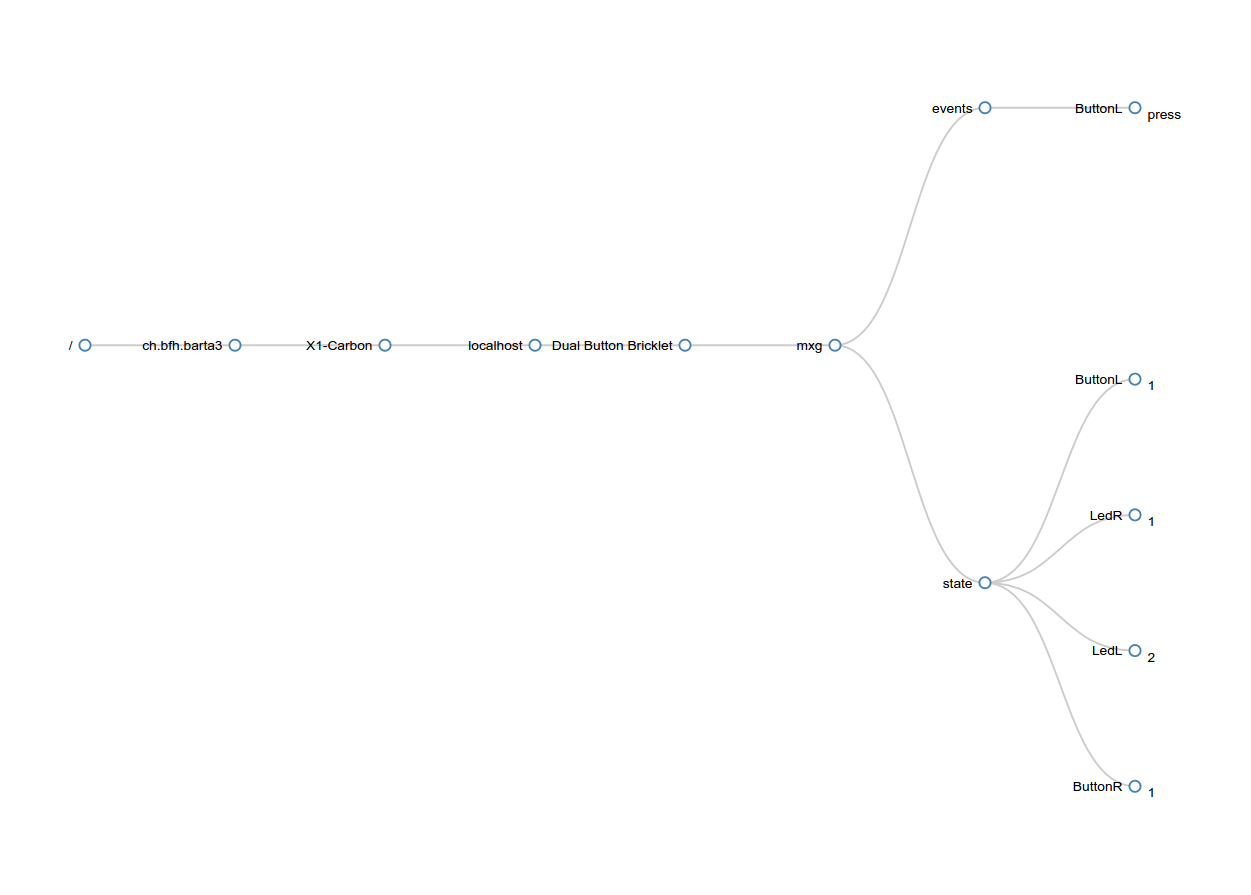
\includegraphics[width=0.8\textwidth]{bilder/TopicHierarchie_Bsp_Dualbutton.png}
	\caption{\label{fig:tempitTopics}Visualisierung MQTT Topics Tinkerforge IR Temperatur Sensor}
\end{figure}

TODO: better diagram

\section{Payload Format}

\subsection{JSON}



\section{Device Description}

Die Beschreibung eines Device enthält die drei Elemente State, Events und Commands.

\textbf{State} \\
Die State Informationen des Devices werden als Key-Value Paare abgebildet. Der Name der Keys muss eindeutig sein.

\textbf{Events} \\
Ein Device muss beschreiben, welche Events es versendet und was darin enthalten ist.
Ein Event ist folgendermassen aufgebaut:
Name, Liste von Attributen als Key-Value Paare.

\textbf{Commands}